\pagestyle{acorde}
\label{acorde}
%\begin{textblock*}{5.625in}(0pt,0pt)%
%\vspace*{-3.5cm}
%\hspace*{-2.77cm}\includegraphics*[width=175.2mm]{./propagandas/IMA.pdf}
%\end{textblock*}
%\pagebreak

\begin{center}
\hspace*{.5cm}
\includegraphics[width=74mm]{./CAPAS/ACORDE_TATIT.jpg}
\end{center}
\hspace*{-7cm}\hrulefill\hspace*{-7cm}
\medskip

\noindent{}Luiz Tatit é professor de linguística, crítico, ensaísta e teórico da canção, além de cancionista. Depois da bem-sucedida atuação no grupo Rumo, um dos experimentos mais vigorosos e relevantes da vanguarda paulista, começa a desenvolver sua carreira solo com o álbum \textit{Felicidade}. Além disso, tem uma série de trabalhos em parcerias, como os que fez com Arrigo Barnabé e Lívia Nestrovski, e o conjunto de shows com José Miguel Wisnik e Arthur Nestrovski.

Seu trabalho na crítica começa a se desenvolver a partir dos anos 80, com a escrita de textos em cadernos culturais, e a publicação do livro \textit{A canção, eficácia e encanto}. Depois se seguiu uma série de outras publicações, entre livros e artigos, \hlc{tendo sempre como objeto central a canção, e como objetivo geral a construção de uma teoria e de uma mediação crítica própria a essa linguagem artística.}

\vfill
\hspace*{-.4cm}\begin{minipage}[c]{.5\linewidth}
\small\textbf{
\hspace*{-.1cm}Editora: Acorde\\
Título: Luiz Tatit: no princípio era o meio\\
Autor: Luís Augusto Fischer\\ 
ISBN: 978-65-994412-9-5\\
Páginas: 135 (provisório)\\
Formato: 13,3x21\,cm\\
Preço: R\$ 53,90 (provisório)\\
}
\end{minipage}
\pagebreak

\begin{center}
\hspace*{-3.6cm}\raisebox{5cm}{\rotatebox[origin=t]{90}{\huge\textbf{Lançamento}}}
\hspace*{3.1cm}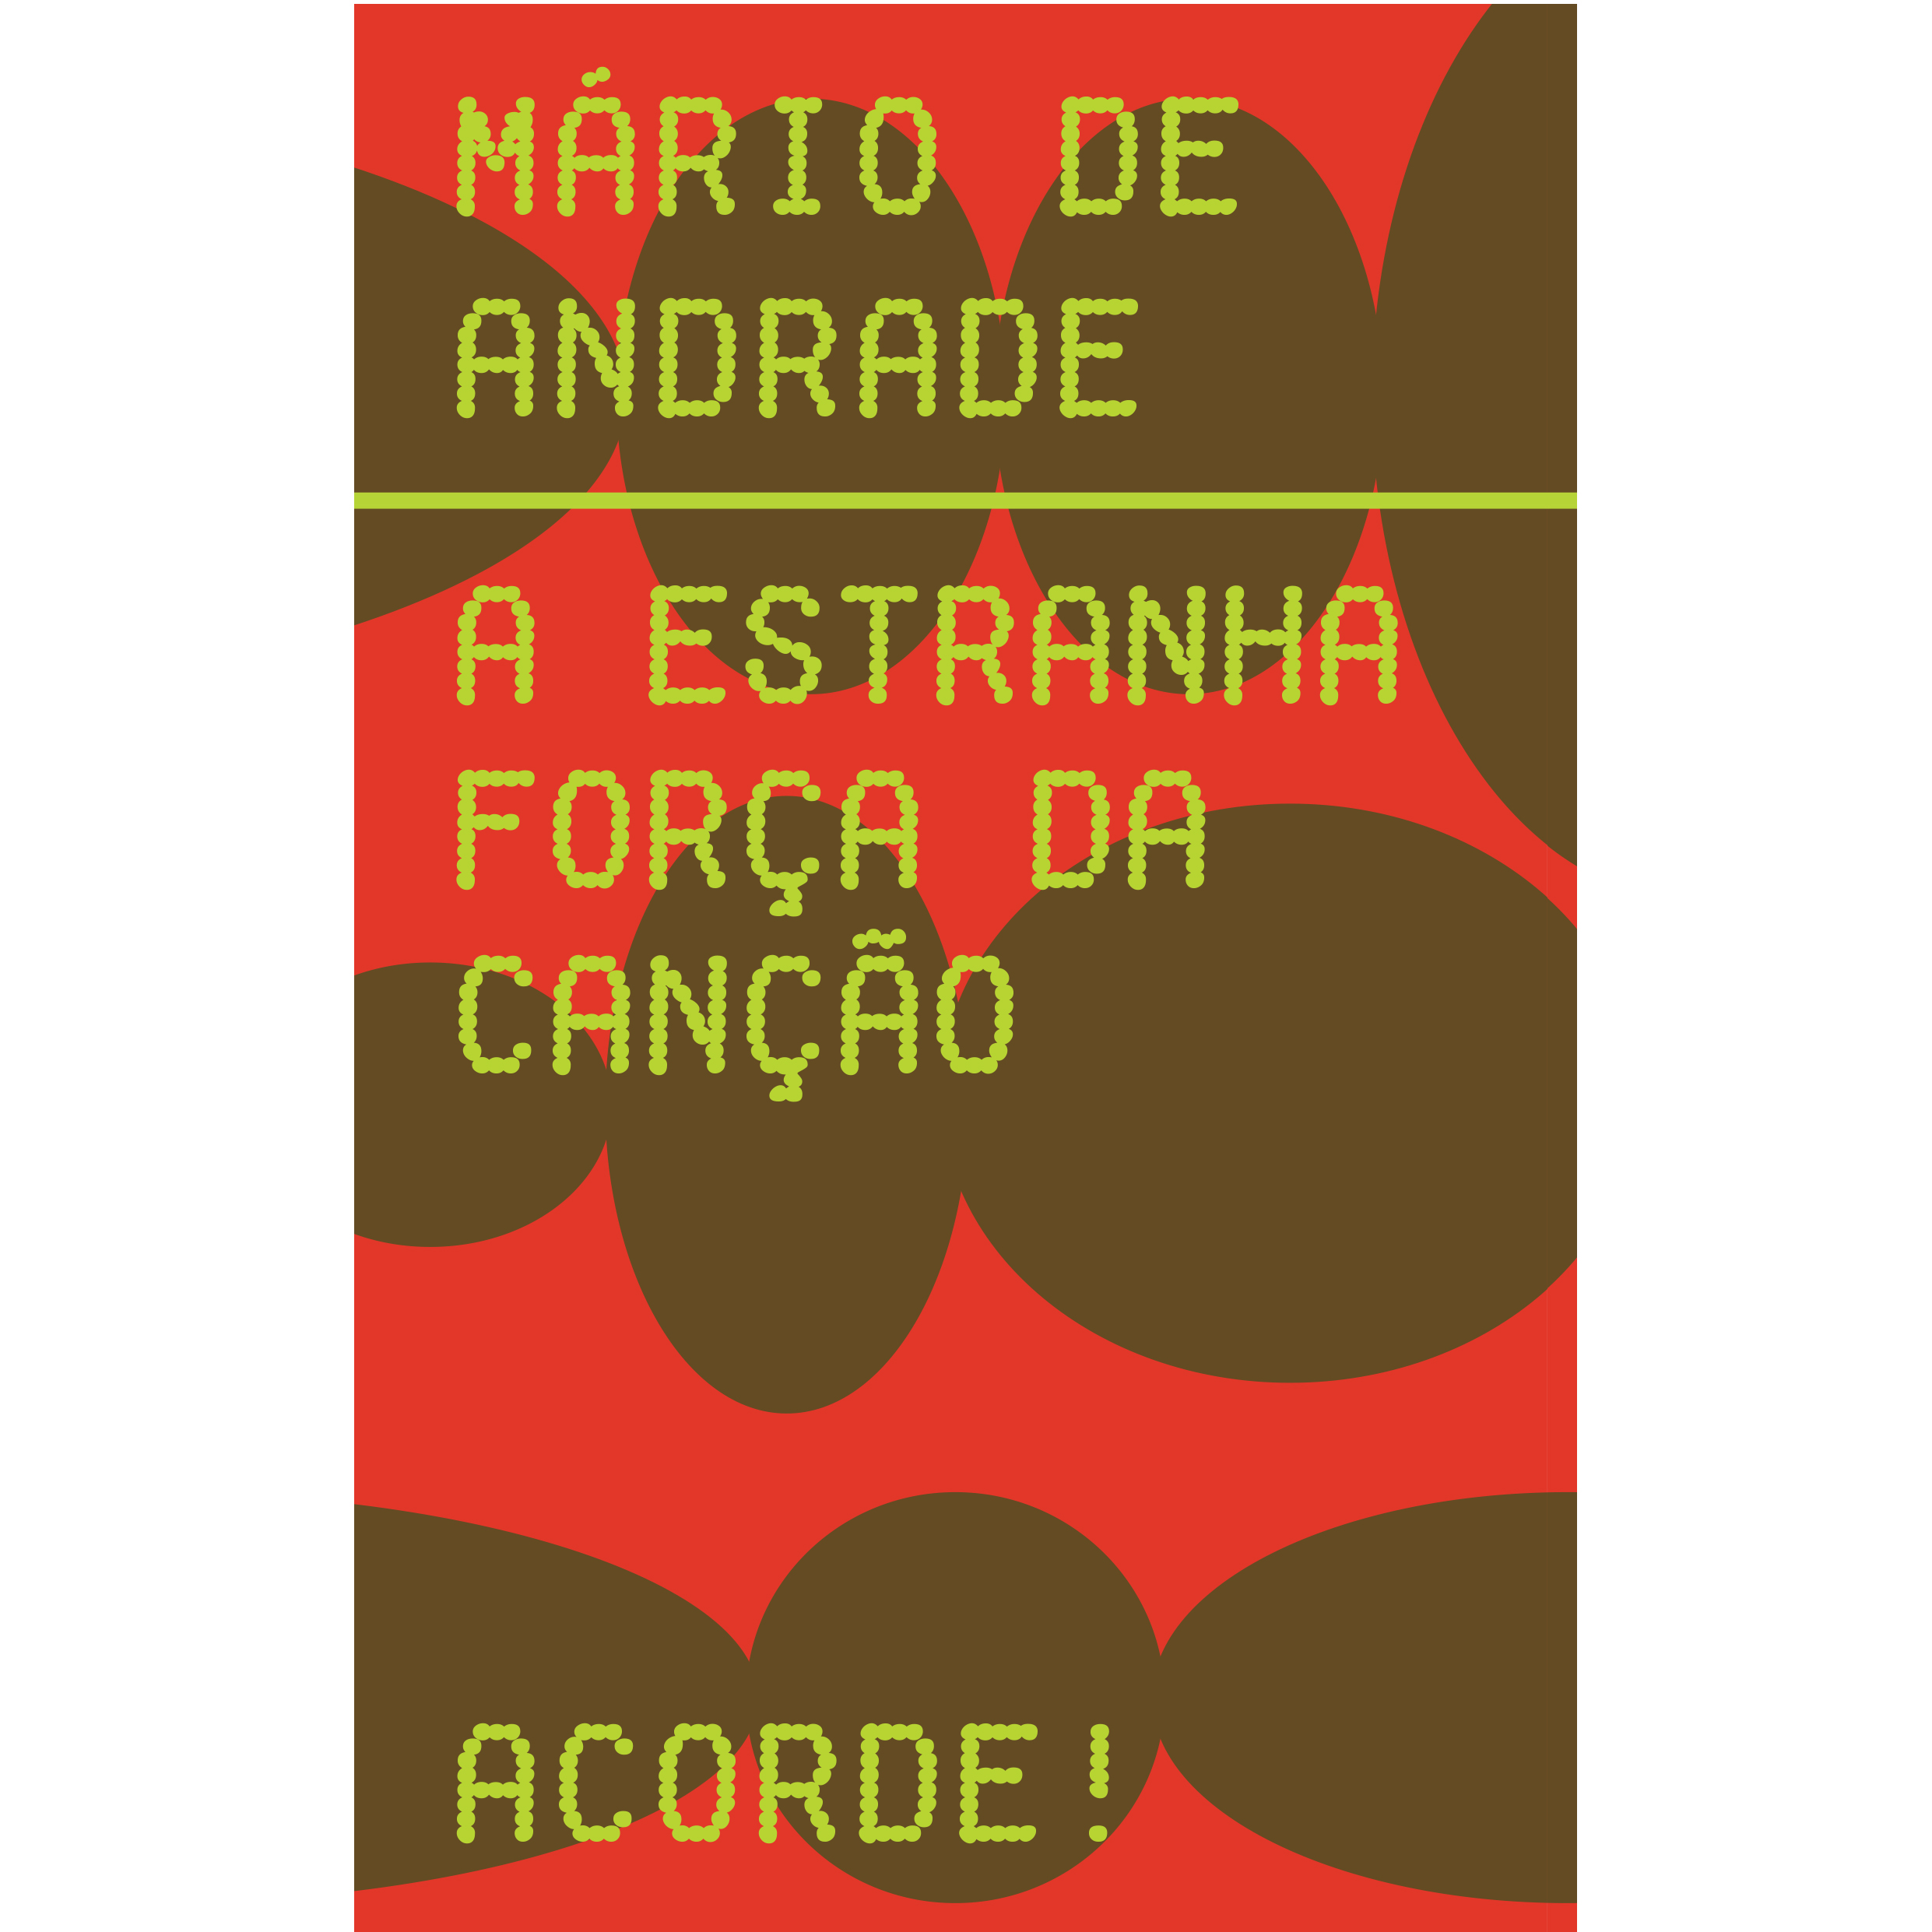
\includegraphics[width=74mm]{./CAPAS/ACORDE_MARIO.jpg}
\end{center}
\hspace*{-7cm}\hrulefill\hspace*{-7cm}
\medskip

\noindent{}Mário viveu entre 1893 e 1945, e sobre o tema da música publicou muito e dispersamente. Foi um músico de formação erudita que desde jovem, em 1916, com 22 para 23 anos, além de professor na área; \hlc{por toda a vida manteve acesa a atenção para os fenômenos musicais não-eruditos, que vão do popular mais elementar, como uma cantiga ancestral de roda, ao mais elaborado}, como a canção gravada em discos, eventualmente orquestrada para músicos que sabiam ler partitura, vendida com sucesso no mercado e validada pelo assobio anônimo. 

Entre os vários pontos extremos desse quadro --- o polo erudito e o popular, tradição escrita e tradição oral, instrumentos de concerto e instrumentos de batuque, campo e cidade, sagrado e profano, individual e grupal ---, mundos inteiros se apresentam e simbolizam a experiência humana em seus múltiplos e contraditórios aspectos, e da mesma forma se cruzam e realimentam, por variados caminhos e com diferentes intensidades.

\vfill
\hspace*{-.4cm}\begin{minipage}[c]{.5\linewidth}
\small\textbf{
\hspace*{-.1cm}Editora: Acorde\\
Título: Mário de Andrade: a estranha\\força da canção\\
Autor: Marcos Lacerda\\ 
ISBN: 978-65-994412-8-8\\
Páginas: 194 (provisório)\\
Formato: 13,3x21\,cm\\
Preço: R\$ 65,90 (provisório)\\
}
\end{minipage}
%\pagebreak

% \vspace*{1.5cm}
% \noindent{}{\nohyphens{\LARGE{Texto}}}
% \bigskip

% \hfill{}\scalebox{.8}{AUTOR}
% \bigskip
% \bigskip
% \bigskip

% \begin{multicols}{2}
% \noindent{}Mussum Ipsum, cacilds vidis litro abertis. Atirei o pau no gatis, per gatis num morreus. Leite de capivaris, leite de mula manquis sem cabeça. Praesent malesuada urna nisi, quis volutpat erat hendrerit non. Nam vulputate dapibus. Suco de cevadiss, é um leite divinis, qui tem lupuliz, matis, aguis e fermentis.

% Tá deprimidis, eu conheço uma cachacis que pode alegrar sua vidis. Suco de cevadiss deixa as pessoas mais interessantis. In elementis mé pra quem é amistosis quis leo. Quem num gosta di mim que vai caçá sua turmis!

% Viva Forevis aptent taciti sociosqu ad litora torquent. Mauris nec dolor in eros commodo tempor. Aenean aliquam molestie leo, vitae iaculis nisl. Posuere libero varius. Nullam a nisl ut ante blandit hendrerit. Aenean sit amet nisi. Vehicula non. Ut sed ex eros. Vivamus sit amet nibh non tellus tristique interdum.

% Em pé sem cair, deitado sem dormir, sentado sem cochilar e fazendo pose. Detraxit consequat et quo num tendi nada. Pra lá , depois divoltis porris, paradis. Per aumento de cachacis, eu reclamis.

% Quem manda na minha terra sou euzis! A ordem dos tratores não altera o pão duris. Paisis, filhis, espiritis santis. Aenean aliquam molestie leo, vitae iaculis nisl.

% Diuretics paradis num copo é motivis de denguis. Mais vale um bebadis conhecidiss, que um alcoolatra anonimis. Sapien in monti palavris qui num significa nadis i pareci latim. Admodum accumsan disputationi eu sit. Vide electram sadipscing et per.

% Manduma pindureta quium dia nois paga. Interagi no mé, cursus quis, vehicula ac nisi. Praesent vel viverra nisi. Mauris aliquet nunc non turpis scelerisque, eget. Casamentiss faiz malandris se pirulitá.

% Quem num gosta di mé, boa gentis num é. Si num tem leite então bota uma pinga aí cumpadi! Todo mundo vê os porris que eu tomo, mas ninguém vê os tombis que eu levo! Cevadis im ampola pa arma uma pindureta.

% \vspace{\baselineskip}
% {\small\fakereceipt{
% \noindent{}Diuretics paradis num copo é motivis de denguis. Mais vale um bebadis conhecidiss, que um alcoolatra anonimis. Sapien in monti palavris qui num significa nadis i pareci latim. Admodum accumsan disputationi eu sit. Vide electram sadipscing et per.
% }}
% \vspace{\baselineskip}

% Mussum Ipsum, cacilds vidis litro abertis. Atirei o pau no gatis, per gatis num morreus. Leite de capivaris, leite de mula manquis sem cabeça. Praesent malesuada urna nisi, quis volutpat erat hendrerit non. Nam vulputate dapibus. Suco de cevadiss, é um leite divinis, qui tem lupuliz, matis, aguis e fermentis.

% Tá deprimidis, eu conheço uma cachacis que pode alegrar sua vidis. Suco de cevadiss deixa as pessoas mais interessantis. In elementis mé pra quem é amistosis quis leo. Quem num gosta di mim que vai caçá sua turmis!

% Viva Forevis aptent taciti sociosqu ad litora torquent. Mauris nec dolor in eros commodo tempor. Aenean aliquam molestie leo, vitae iaculis nisl. Posuere libero varius. Nullam a nisl ut ante blandit hendrerit. Aenean sit amet nisi. Vehicula non. Ut sed ex eros. Vivamus sit amet nibh non tellus tristique interdum.

% Em pé sem cair, deitado sem dormir, sentado sem cochilar e fazendo pose. Detraxit consequat et quo num tendi nada. Pra lá , depois divoltis porris, paradis. Per aumento de cachacis, eu reclamis.

% Quem manda na minha terra sou euzis! A ordem dos tratores não altera o pão duris. Paisis, filhis, espiritis santis. Aenean aliquam molestie leo, vitae iaculis nisl.

% Diuretics paradis num copo é motivis de denguis. Mais vale um bebadis conhecidiss, que um alcoolatra anonimis. Sapien in monti palavris qui num significa nadis i pareci latim. Admodum accumsan disputationi eu sit. Vide electram sadipscing et per.

% Manduma pindureta quium dia nois paga. Interagi no mé, cursus quis, vehicula ac nisi. Praesent vel viverra nisi. Mauris aliquet nunc non turpis scelerisque, eget. Casamentiss faiz malandris se pirulitá.

% Quem num gosta di mé, boa gentis num é. Si num tem leite então bota uma pinga aí cumpadi! Todo mundo vê os porris que eu tomo, mas ninguém vê os tombis que eu levo! Cevadis im ampola pa arma uma pindureta.

% \bigskip
% \noindent{}\textcolor{gray}{\footnotesize\slsc{\textls[-15]{Texto tal tal e tal.}}}
% \end{multicols}

% \pagebreak
% \pagestyle{acordecat}
% \begin{multicols}{2}
% \begin{enumerate}
% \raggedright\nohyphens{

% }
% \end{enumerate}
% \end{multicols}

\pagebreak